\documentclass[11pt]{article}
\usepackage[margin=2.2cm]{geometry}
\usepackage{amsmath,amssymb,listings}
\usepackage{booktabs}
\usepackage{xurl}
\usepackage{xcolor}
\usepackage[colorlinks=true,linkcolor=blue!50!black,citecolor=blue!50!black,urlcolor=blue!50!black]{hyperref}
\usepackage{orcidlink}
\usepackage{tikz}
\usetikzlibrary{positioning,arrows.meta}

\lstset{
    language=Python,
    basicstyle=\ttfamily\small,
    keywordstyle=\color{blue!60!black}\bfseries,
    stringstyle=\color{green!45!black},
    commentstyle=\color{gray}\itshape,
    breaklines=true,
    frame=single,
    framerule=0.3pt,
    xleftmargin=1em,
    columns=fullflexible,
    keepspaces=true,
    showstringspaces=false
}
\lstdefinelanguage{crustc}{
    language=C,
    morekeywords={assert,invariant,variant}
}

\newcommand{\code}[1]{\texttt{#1}}

\title{Proofs Small Enough to Read:\\
Kernel Contracts from \LaTeX{} Theorems to Compiler Decisions}
\author{Brent S. Hartshorn \orcidlink{0009-0004-2853-655X} \small \url{brenthartshorn@proton.me}}

\begin{document}
\maketitle

\begin{abstract}
In September 2026 a computer-checked proof of Fermat's Last Theorem and a
Lean-formalized proof of blowup in the forced Navier--Stokes equations were
announced within days of each other, and both are believed because a kernel
checked them. This paper applies that discipline at the other end of the
scale. A Calculus of Constructions micro-kernel with no axioms, 
is given an imperative language---assignment, branches, bounded
loops, and \code{while} with an explicit variant---compiled by symbolic
execution into kernel terms. Contracts are decidable propositions,
$\code{Holds}\ b := \code{Eq}\ \code{Bool}\ b\ \code{true}$, about the very
expression a runtime check would evaluate. A \code{while} loop raises four
obligations, one of them the soundness of its own lowering, and termination
is proved for every starting state. Records and a state invariant give a model
of an seL4-style OS whose routing layer carries contracts that hold for every
input. A bridge to Crust, a self-contained C/C++/Rust toolchain, settles its
source-level contracts in the kernel; building it found two of Crust's passes
reading one contract two ways. Finally a certificate changes generated code: a
SIMD kernel's scalar remainder is omitted on it, 
and a contract proven at every call site downgrades 80\% of the
memory-safety checks in a leaf initializer while the check it leaves still
catches an overflow.
\end{abstract}

\section{Introduction}

Anthropic (2026) reported that Claude, working largely
autonomously over eleven days, had produced the first end-to-end
computer-checked proof of Fermat's Last Theorem: thirteen million lines of
Lean, 29{,}500 intermediate theorems, and---in Kevin Buzzard's words---``no
assumptions other than the axioms of mathematics''
\cite{anthropic2026flt,newscientist2026flt,nature2026flt}. Four days later
OpenAI reported a proof that the Navier--Stokes equations, under a smooth
applied force, can develop a singularity in finite time, released with a Lean
formalization whose verification took a further seventeen hours
\cite{openai2026ns}; the unforced problem remains open \cite{mcgreivy2026}.

What the two share is not their subject but their epistemology. Nobody has
read thirteen million lines of Lean. The proof is believed because a kernel
checked it, and the kernel is trusted because it is small---the move the
Simons Foundation called ``from trust to verification'' \cite{simons2026},
and that Buzzard, watching AI systems settle Erd\H{o}s problems faster than
they could be posed, called being ``outcounterexampled''
\cite{buzzard2026counter}.

This paper is about that shift at the other end of the scale. 
Follwing from a \LaTeX{} subset to Python
with a dependent-type micro-kernel that checks proofs about Python functions
\cite{hartshorn2026rosetta}, and a C/C++/Rust toolchain small enough to read,
whose memory-safety instrumentation omits what the compiler can prove away
\cite{hartshorn2026memsafe,hartshorn2026subtraction}. The kernel could check
a proof term; the compiler could decide, by hand-written dataflow, that a
check was unnecessary; neither talked to the other. Now they do
(Figure~\ref{fig:pipeline}), and the contribution is the chain between them:
an imperative fragment compiled into ordinary kernel terms
(\S\ref{sec:fragment}); a \code{while} rule that states the soundness of its
own lowering as an obligation, and termination proved for every state
(\S\ref{sec:loops}); records, a state invariant, and composition by chaining
proofs (\S\ref{sec:state}); a model of an seL4-style OS's routing layer, all
four functions of which carry contracts that hold for every input
(\S\ref{sec:os}); a bridge to Crust that found two passes reading one contract
two ways (\S\ref{sec:crust}); and generated code that depends on a proof
(\S\ref{sec:codegen}).

\begin{figure}[h]
\centering
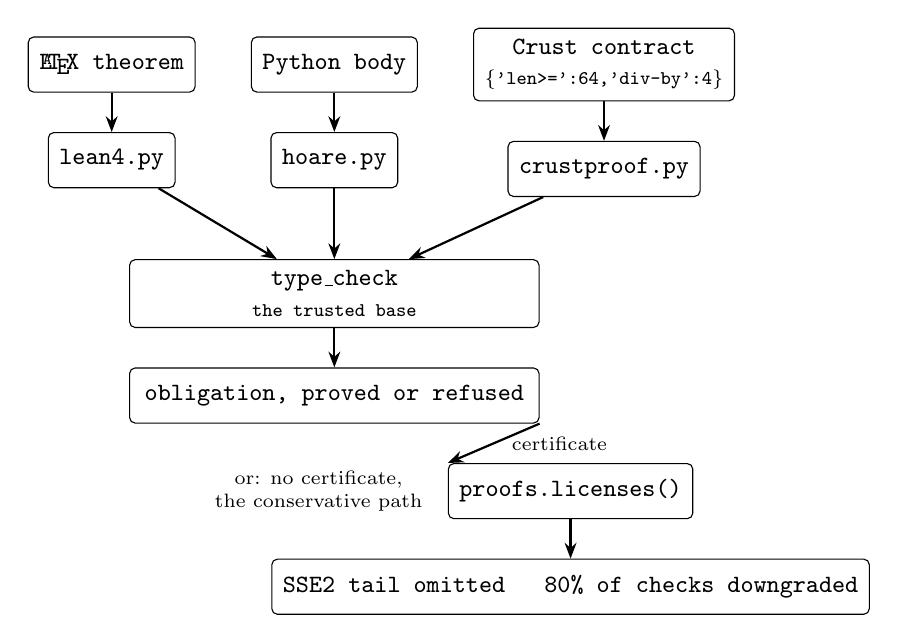
\begin{tikzpicture}[
  node distance=5mm and 7mm,
  box/.style={draw,rounded corners=2pt,inner sep=4pt,font=\small\ttfamily,minimum height=7mm,align=center},
  lab/.style={font=\scriptsize,align=center},
  arr/.style={-{Stealth[length=2mm]},thick}]
  \node[box] (latex) {\LaTeX{} theorem};
  \node[box,right=of latex] (py) {Python body};
  \node[box,right=of py] (crust) {Crust contract\\{\scriptsize\{'len>=':64,'div-by':4\}}};
  \node[box,below=of latex] (l4) {lean4.py};
  \node[box,below=of py] (hoare) {hoare.py};
  \node[box,below=of crust] (cp) {crustproof.py};
  \node[box,below=9mm of hoare,minimum width=52mm] (kernel) {type\_check\\{\scriptsize the trusted base}};
  \node[box,below=of kernel,minimum width=52mm] (obl) {obligation, proved or refused};
  \node[box,below=of obl,xshift=30mm] (lic) {proofs.licenses()};
  \node[box,below=of lic] (gen) {SSE2 tail omitted \quad 80\% of checks downgraded};
  \draw[arr] (latex)--(l4); \draw[arr] (py)--(hoare); \draw[arr] (crust)--(cp);
  \draw[arr] (l4)--(kernel); \draw[arr] (hoare)--(kernel); \draw[arr] (cp)--(kernel);
  \draw[arr] (kernel)--(obl);
  \draw[arr] (obl.south east)--(lic.north west) node[lab,midway,right=1mm] {certificate};
  \draw[arr] (lic)--(gen);
  \node[lab,left=2mm of lic] {or: no certificate,\\the conservative path};
\end{tikzpicture}
\caption{Three front ends, one checker, and the decision a compiler makes on the
strength of what it checked.}
\label{fig:pipeline}
\end{figure}

Two disclaimers. The micro-kernel is named \code{lean4.py} for the discipline
it follows and the statement language it reads, not because it is Lean; it is
a Calculus of Constructions checker with de Bruijn indices and an untrusted
elaborator. And the OS is a model: the scheme layer of \code{crustos} and the
shape of a scheduler are modelled and proved about; nothing boots.

\section{Background}
\label{sec:background}

\subsection{RosettaMath and the micro-kernel}

RosettaMath \cite{hartshorn2026rosetta} is a self-hosting translator from a
subset of \LaTeX{} to Python, built for the gap between the notation
mathematics is written in and the language a student can run. Alongside it is
\code{lean4.py}, a Calculus of Constructions \cite{coquand1988} checker in
which the theorem statements are written in that same \LaTeX{} subset:

\begin{lstlisting}
@theorem(r'\forall x \in \text{Nat}, x = x')
def reflexivity(x: 'Nat'):
    return refl(x)
\end{lstlisting}

The decorator compiles the function to a kernel term, reads the statement as a
type, and requires the two to agree definitionally. This inverts the Xena
project's bridge, which rendered Lean proofs \emph{into} \LaTeX{}
\cite{massot2019,massot2024}: here \LaTeX{} is the input and the thing proved
is a Python function. It is not Lean \cite{demoura2021}; it is a kernel of the
same design, small enough to be a teaching object.

The front end accepted exactly one \code{return}---enough for a proof term,
not for a program. The previous paper closed by naming the next step: make the
statement language the contract language of Crust, so that a contract is a
$\Pi$-type and the obligation a theorem the kernel checks. ``This is future
work, and we do not claim more than the shape of it here.'' This paper is that
work.

\subsection{Crust and its contracts}

Crust \cite{hartshorn2026subtraction} is a C, C++ and Rust toolchain that owns
its whole stack: every source language lowers to plain C, and one
self-contained backend takes C to machine code, with no external compiler. Its
memory-safety paper \cite{hartshorn2026memsafe} argues that uniform
instrumentation asks questions the compiler already knows the answers to, so a
whole-program view should prove most checks away before they are emitted.

Contracts already exist in Crust's C. A source pre-pass lifts \code{assert}
clauses out of the region between a function's parameter list and its body,
blanks them space-for-space so byte offsets are preserved, and hands the
result downstream as structured metadata:

\begin{lstlisting}[language=crustc]
int calc_sum(int *ptr, unsigned int len)
assert len(ptr) >= 64
assert not len(ptr) % 4
{ ... }
\end{lstlisting}

becomes \code{\{'ptr': \{'len>=': 64, 'div-by': 4\}\}}, which four
whole-program passes consume: call-site violations become compile errors,
proven alignment lets a reduction drop its scalar remainder, a declared core
partitions the register file, and the memory-safety instrumentation omits what
it can prove. The passes share a discipline---a proof that fails degrades to
the conservative path---but, as \S\ref{sec:crust} reports, not a definition.

\section{The kernel, and three measured fixes}
\label{sec:kernel}

A term is a universe, a free or bound variable, an application, a
metavariable, a $\Pi$ or a $\lambda$, over de Bruijn indices. Equality is
structural on the de Bruijn form, so it is $\alpha$-equivalence for free.
Reduction is $\beta$, $\delta$ (unfolding a definition) and $\iota$ (a
recursor meeting a constructor). \code{type\_check} is the whole trusted base;
the elaborator, which fills implicit arguments by Miller pattern unification,
is untrusted, and the kernel re-checks its output from scratch.
\code{inductive()} generates two recursors per family, \code{T.rec} into
\code{Type 0} and \code{T.ind} into \code{Prop}, because there is no universe
polymorphism. One restriction is stated rather than hidden: a recursive
argument is refused in a family with indices, since the induction hypothesis
would have to name that occurrence's indices.

The imperative fragment was blocked before it began. \code{leb 20 30} did not
terminate. The cause took three passes, and each was measured before it was
fixed (Table~\ref{tab:kernel-perf}).

\begin{table}[h]
\centering
\small
\begin{tabular}{p{4.2cm} p{5.6cm} p{5.2cm}}
\toprule
symptom & cause & fix \\
\midrule
cost $2^n$; normal forms $14n+3$ &
pure recomputation &
memoise \code{normalize} per environment generation \\
still exponential &
substitution \emph{shares} the inserted term, so a body using its argument
three times builds a DAG with $3^n$ paths and $O(n)$ nodes; hashing a nested
tuple walks paths &
structural keys become interned integers \\
4.5M \code{shift} and 2.7M \code{instantiate} calls &
the DAG re-expanded into a tree on every substitution &
memoise the de Bruijn rewrites, so a hit returns the same object \\
\bottomrule
\end{tabular}
\caption{Three fixes to \code{normalize}. \code{modb 12}: 134\,s to 0.003\,s.
\code{modb 32}: never, to 0.046\,s. Each was gated on byte-identical selftest
and demo output.}
\label{tab:kernel-perf}
\end{table}

Keying the caches on the structural key silently reprinted \code{symm}'s type, turning
\code{\{a : A\}} into \code{a : A}: the structural key is blind to binder
hints and implicitness---that is what makes it $\alpha$-equivalence---but the
rewrites carry both through. A second key, \code{fullkey()}, draws the line
where the rewrites do.

\subsection{The statement language, read backwards}
\label{sec:roundtrip}

The \LaTeX{} subset was an input language only. \code{type2latex} makes it an
output language as well, and the property that makes that worth having is
$\code{latex2type}(\code{type2latex}(t)) = t$ for every term the kernel
checks. It is written against the parser rather than against taste: every
shape it emits is emitted because the parser accepts it, and anything the
parser could not read back is refused with the reason---a hole, a loose index,
\code{Type 1}, a name like \code{N} that the reader would alias away---rather
than approximated. The existing pretty-printer is not this function and cannot
become it: it prints \code{Type 1}, \code{?A7}, $\lambda$ and \code{x'}, none
of which the reader takes.

Two places where the term does not determine the text. A binder's name is free
to change, since the structural key ignores name hints, but only within what
the lexer can read: \code{Nat} lexes as three tokens and a binder name is
taken as one, so a bound name must be a single letter, and the letter chosen
must also avoid the free names of the body or the reader would abstract two
variables into one. And \code{a = b} is written only when the parser's
recovery of \code{Eq}'s carrier---from the binder that introduced an
operand---would return this very carrier; otherwise the application is written
out, which always reads back.

\textbf{The printer found what the language was missing.} Of the 91
declarations the environment holds, five had types it refused, and they are
most of Table~\ref{tab:lemmas}: \code{snoc\_le}, \code{stuck},
\code{fold\_preserves}, \code{fold\_terminates},
\code{loop\_preserves}. Every one for the same reason, a $\lambda$ inside a
\emph{type}: an induction motive in the first, the \code{Nat.rec} of
\S\ref{sec:loops} in the rest. Normalising removes neither. So the subset gained $\lambda x : A,\ b$ on both sides at
once, which is what keeps the two inverse; every type and every value in that
environment, 141 terms, now round-trips, and
Appendix~\ref{sec:appendix} is written in \LaTeX{} on the strength of it. A
latent bug came out with it: the parser stopped an application at a
\code{\textbackslash forall} but an atom did not, so an arrow whose right side
began with one read the binder as a variable \emph{named} \code{forall}, and
failed later, somewhere confusing.

\section{Contracts as decidable propositions}
\label{sec:contracts}

The natural encoding of $\le$, an inductive family, is refused by
\code{inductive()}, and the refusal is deliberate. Rather than route around
it:
\[
  \code{Holds}\ b \;:=\; \code{Eq}\ \code{Bool}\ b\ \code{true}.
\]
A contract is a \code{Bool}-valued expression, and the proposition is that it
computes to \code{true}. Every bound Crust's \code{extensions.py} parses is
already decidable, because a contract a compiler cannot \emph{check} is no use
to it. So the proposition is about the same expression the runtime check would
evaluate, and the proof is what licenses deleting the check. Closed instances
need no proof at all: they compute, and \code{refl} is the proof.

\section{The imperative fragment}
\label{sec:fragment}

\code{PythonToLean} accepts exactly one \code{return}. \code{ImpToLean}
accepts a body. It is symbolic execution, not a semantics: there is no state
type, no variable type, no big-step relation. The store is a dictionary from a
variable to the term it currently holds, so assignment is a substitution
performed in the compiler rather than a \code{let} the kernel would have to
understand (Table~\ref{tab:lowering}). Nothing here is trusted; whatever it
produces is handed to \code{type\_check}, which knows nothing of Python.

\begin{table}[h]
\centering
\small
\begin{tabular}{ll}
\toprule
Python & becomes \\
\midrule
\code{v = e} & substitution into the store \\
\code{if c: \ldots else: \ldots} & \code{ite} per assigned variable \\
\code{for i in range(n)} & \code{Nat.rec}---the fold it always was \\
\code{while c} with a variant & iterating a guarded step; fuel is the variant on entry \\
several loop-carried variables & packed into a right-nested \code{Prod} \\
\code{c.field = e} & \code{c = Record.with\_field c e} \\
\code{out: 'Array' = []} & \code{nil} at the annotation's element type \\
\bottomrule
\end{tabular}
\caption{The lowering.}
\label{tab:lowering}
\end{table}

\subsection{The \code{while} rule}
\label{sec:whilerule}

A while loop terminates for a reason the text does not state, so lowering one
unannotated means inventing a variant---a guess where a guess is an unproved
theorem. An annotation supplies it:

\begin{lstlisting}
while c.current < c.nthreads:
    assert invariant(c.current <= c.nthreads)
    assert variant(c.nthreads - c.current)
    c.current = c.current + 1
\end{lstlisting}

The condition, invariant, variant and one pass are each named as functions of
the state, and the fold is built from those names, which is what lets a
general lemma about folds apply to a particular loop. Four obligations are
raised (Table~\ref{tab:while}), and the soundness of the lowering is one of
them: there is no metatheorem in a comment saying the fold equals the loop.

\begin{table}[h]
\centering
\small
\begin{tabular}{ll}
\toprule
obligation & says \\
\midrule
\code{progress} & the condition really is false when the fold is done \\
\code{invariant holds on entry} & $\code{Holds}\,(\mathit{inv}\ s_0)$ \\
\code{invariant is preserved} & $\forall s,\ \code{Holds}\,(\mathit{inv}\ s) \to \code{Holds}\,(\mathit{cond}\ s) \to \code{Holds}\,(\mathit{inv}\ (\mathit{pass}\ s))$ \\
\code{variant decreases} & $\forall s,\ \ldots \to \code{Holds}\,(\code{ltb}\ (\mathit{rank}\ (\mathit{pass}\ s))\ (\mathit{rank}\ s))$ \\
\bottomrule
\end{tabular}
\caption{What a \code{while} loop owes.}
\label{tab:while}
\end{table}

Two hypotheses, not one \code{andb}: a case split on the condition then has
$\code{Holds}\ \code{true}$ to hand, which \code{refl} proves, whereas
$\code{Holds}\,(\code{andb}\ I\ \code{true})$ with symbolic $I$ has nothing to
reduce. Only one form composes; the fact was found by failing to prove
\code{guarded} with the other.

\subsection{What is refused}

Roughly a third of the fragment's 157 checks are refusals, each pinned to its
reason: \code{while} without a variant; \code{return} inside a loop (a fold
cannot stop early) or a branch (the join would have to know which ran); an
iterable that is not \code{range(n)}; an unannotated parameter; a variable
assigned on one branch only, or changing type; division; a postcondition that
is not \code{Bool}; an empty list with no annotation; a missing field. Once the
state invariant exists: a syscall that can break it, a suffix that breaks it,
a variant that does not come down, and a field name never bound---which raises
at once rather than falling through, because a mistake in the caller's own
lemma is theirs to see. The refusals are the deliverable as much as the
acceptances: a fragment that accepted \code{while} without a variant would be
lowering a guess.

\section{Loops, proved}
\label{sec:loops}

\subsection{Two definitions that computed the right answer}

$\code{iter}\ (n{+}1)\ s$ is $\code{iter}\ n\ (\code{step}\ s)$, not
$\code{step}\ (\code{iter}\ n\ s)$. Both compute the same thing, but the
variant comes down on the \emph{first} pass, so that is where an induction on
termination has to be able to look. Likewise \code{sub} recurses on its first
argument, so $\code{sub}\ (m{+}1)\ (n{+}1)$ is $\code{sub}\ m\ n$ by
definition; iterating \code{pred} on the second argument gives the same
numbers and no such equation, and leaves a proof about an $n - i$ variant
with nothing to induct on. A definition that computes the right answer can
still be the wrong definition to reason about.

\subsection{The lemmas}

\begin{table}[h]
\centering
\small
\begin{tabular}{ll}
\toprule
lemma & proved by \\
\midrule
$\code{absurd} : \forall C{:}\code{Prop},\ \code{Holds}\ \code{false} \to C$ & \code{Eq.ind} into a motive reading \code{true} as the goal \\
\code{leb\_refl}, \code{leb\_succ} & induction \\
\code{leb\_trans} & induction on the first argument, case split on the other two \\
\code{sub\_le}, \code{sub\_lt} & induction \\
\code{snoc\_le} & induction on the list, case split on the bound \\
\code{andb\_both}, \code{andb\_left}, \code{andb\_right} & \code{Bool.ind} \\
\code{guarded} & a case split on the condition \\
\code{fold\_preserves} & induction on the number of passes \\
\code{loop\_preserves} & the two composed \\
\code{stuck} & once the condition is false, iterating changes nothing \\
\code{fold\_terminates} & the variant bounds the number of passes \\
\bottomrule
\end{tabular}
\caption{Everything a \code{while} loop appeals to. None is an axiom.}
\label{tab:lemmas}
\end{table}

\code{fold\_terminates} is the one that matters most. \code{progress} used to
be discharged only at concrete values, which checks the examples and says
nothing about the rest. It is now proved for every starting state, and the
environment in which it is proved contains 91 declarations---7 inductive
families, 10 constructors, 14 recursors, 59 definitions---and no axioms.

\section{State: records, an invariant, composition}
\label{sec:state}

A single-constructor inductive is a record; what \code{inductive()} does not
give is names. \code{record(env, name, fields)} generates, per field,
$\code{Name.field} : \code{Name} \to T$ and $\code{Name.with\_field} :
\code{Name} \to T \to \code{Name}$, both by $\iota$ on the one constructor, so
both compute. In the fragment, \code{c.ticks = c.ticks + 1} lowers to
$\code{Context.with\_ticks}\ c\ (\code{add}\ (\code{Context.ticks}\ c)\ 1)$.
Nothing is mutated: a syscall takes a context and returns one, which is what
makes state threadable through a sequence of them.

\code{state\_invariant(env, 'Context', 'c.current <= c.nthreads')} defines
$\code{Context.invariant} : \code{Context} \to \code{Bool}$, a property of the
state rather than of any operation, which is the seL4 shape \cite{klein2009}.
\code{@procedure(preserves='Context')} then lets a body assume it and obliges
the syscall to hand it on:
\[
  \forall c,\ \code{Holds}\,(I\ c) \to \code{Holds}\,(I\ (\code{tick}\ c)).
\]

\textbf{Composition chains proofs rather than re-proving.} If $f$ hands the
invariant on and $g$ hands it on, then $g \circ f$ does, and the term that
says so is the two proofs applied in turn:
\[
  \lambda c\ h.\ \mathit{tick}_{\mathrm{pf}}\ (\code{enqueue}\ (\code{tick}\ c))\
  (\mathit{enqueue}_{\mathrm{pf}}\ (\code{tick}\ c)\ (\mathit{tick}_{\mathrm{pf}}\ c\ h)).
\]
The kernel checks the chain.

\textbf{The sequence rule.} A procedure with a loop is three steps---before,
the loop, after---and each must hand the invariant on. The suffix is recovered
as a function of the loop's result by \code{replace\_subterm}, safe because
the target is always an applied loop name with no bound variables of its own.
Segments are named and skipped when definitionally the identity. A correct
loop followed by one increment too many is refused at exactly the right
place:
\begin{quote}\small\ttfamily
what runs after the loop in bad\_suffix changes what the Context invariant
reads, so the hypothesis going in is not a proof of the conclusion coming out.
\end{quote}
A whole-procedure failure would have been much less useful.

\subsection{Why every proof goes through a case split}
\label{sec:casesplit}

$\code{Context.current}\ (\code{Context.with\_ticks}\ c\ v)$ does not reduce
on a symbolic $c$: until the record is known to be built by its constructor,
$\iota$ has nothing to fire on. So even an operation that plainly leaves a
field alone has nothing to compute with. One split on the one constructor
unsticks every projection at once. The subject need not be a record: a loop
carrying two variables carries a \code{Prod}, and the split that unsticks a
record's projections unsticks \code{fst} and \code{snd} for the same reason.

\section{The OS model}
\label{sec:os}

Crust's \code{crustos} is a Redox-shaped OS model in which every resource is a
URL and an \code{open} is routed to whichever \emph{scheme} claims the prefix.
The routing lives in \code{crustos/schemes.py}, in RPython, because it is text
handling and table lookup---which is also what the fragment had to learn to
read.

\code{Context} has six fields: \code{frames}, \code{queue}, \code{schemes},
\code{current}, \code{nthreads}, \code{ticks}. \code{List} is polymorphic, so a
byte string is $\code{List}\ \code{Nat}$ and a list of them is
$\code{List}\ (\code{List}\ \code{Nat})$; on that, \code{find}, \code{take},
\code{drop}, \code{eqs}, \code{split}, \code{append}, \code{snoc} and
\code{rev}. \code{find} returning the length when the separator is absent is
how \code{str.find}'s $-1$ is expressed without a negative number \code{Nat}
does not have. All four public functions of \code{schemes.py} are modelled from
the real source, prefix routing included (Table~\ref{tab:routing}); \code{fil:}
does not route to \code{file}, because \code{eqs} is equality and not prefix
matching, and that distinction is the whole of the routing bug one would want
caught.

\begin{table}[h]
\centering
\small
\begin{tabular}{lll}
\toprule
URL & \code{scheme\_of} & \code{path\_of} \\
\midrule
\code{sys:boot} & 0 & \code{boot} \\
\code{file:/etc/passwd} & 2 & \code{/etc/passwd} \\
\code{gpu:0} & 6 & \code{0} \\
\code{nope:/x} & 7 (sentinel) & \code{/x} \\
\code{/etc/passwd} & 7 & \code{/etc/passwd} \\
\bottomrule
\end{tabular}
\caption{The model agrees with \code{crustos/schemes.py} on every case,
including the absent colon.}
\label{tab:routing}
\end{table}

The contracts are the safety-relevant ones, and all four are proved:
\code{scheme\_of}'s returned index never leaves the scheme table;
\code{path\_of}'s result never grows; \code{route\_all} returns one id per
URL, in order; and \code{accepted}'s result is never longer than its input,
\emph{for every input}.

\subsection{\code{accepted}, end to end}
\label{sec:accepted}

\begin{lstlisting}
@procedure(ensures=['len(result) <= len(split(urls, 44))'])
def accepted(names: 'Strs', urls: 'Bytes') -> 'Array':
    parts = split(urls, 44)
    out: 'Array' = []
    i = 0
    while i < len(parts):
        assert invariant(len(out) <= i and i <= len(parts))
        assert variant(len(parts) - i)
        if scheme_of(names, parts[i]) < len(names):
            out = snoc(out, i)
        i = i + 1
    return out
\end{lstlisting}

The invariant is a conjunction because \code{i <= len(parts)} alone gives
termination and not the result. Entry computes, whatever the input.
Preservation splits on the \code{Prod} the loop carries and then on the
\code{ite} the \code{if} left behind: an accepted URL grows the list by one as
$i$ grows (\code{snoc\_le}); a rejected one moves only $i$
(\code{leb\_trans}, \code{leb\_succ}); \code{andb\_both} rejoins the halves.
The variant is \code{sub\_lt}. \code{progress\_by\_loop} gives termination
for every input, and \code{invariant\_at\_exit} gives the invariant at the
value the loop produced, from which the postcondition follows:
\[
  \forall\,\mathit{names}\ \mathit{urls},\
  \code{Holds}\,(\code{leb}\ (\code{len}\ (\code{accepted}\ \mathit{names}\ \mathit{urls}))\
  (\code{len}\ (\code{split}\ \mathit{urls}\ 44))).
\]
One utility was load-bearing: \code{normalize} is all or nothing, and asked
to look inside the invariant it also unfolds \code{andb} and \code{ite} into
their recursors, leaving no conjunction to take apart. \code{unfold} expands
only the definitions it is told to.

\section{Integration with Crust}
\label{sec:crust}

\code{crustproof.py} turns a Crust contract into a term of type
$\code{Nat} \to \code{Bool}$: \code{\{'len>=': 64, 'div-by': 4\}} becomes
$\code{andb}\ (\code{dvdb}\ 4\ n)\ (\code{leb}\ 64\ n)$. At a known length it
reduces, and when it reduces to \code{true} a proof term is built and
type-checked.

\subsection{What the differential test found}

Crust's two consumers read one contract two ways.
\code{simd\_contracts.\_satisfies} conjoined every clause;
\code{contracts.\_violates} returned on the first clause present. For the
contract in Crust's own SIMD documentation, a length of 70 cleared
\code{len>=} so the \code{div-by} was never looked at: the call compiled,
while \code{simd\_contracts} correctly refused to prove it and kept the scalar
tail. The pass that reports errors was the lenient one. Over a grid of six
contracts and 130 lengths, 110 of 780 cases differed, all of them
multi-clause. Crust now has one reading, in \code{shivyc/proofs.py}, which
both passes call and which raises on a clause it cannot read rather than
skipping it; the diagnostic names the clause the length actually breaks, which
the first-clause reading could not do. \code{crustproof.py} asserts the kernel
agrees with both passes on every case and pins the old reading as a
regression.

\subsection{Literals}

Certification is on by default. It was not, because settling a contract at
length 64 took 1.35\,s and at 1024 took 43\,s: the kernel's numerals are unary,
and the cost grew with the length rather than the size of the number. A
computation rule is now attached to nine definitions that fires only when the
arguments have already reduced to numerals; anything else falls through to
ordinary $\delta$, so every proof by induction is untouched. This is an
extension of the trusted base---Lean does the same for \code{Nat}, for the
same reason---and what keeps it honest is a differential test of each
accelerator against its definition. That test earned its place at once:
$\code{modb}\ n\ 0$ is $n$, because the definition counts up and never meets a
zero divisor to reset at, and the first accelerator said $0$.

\begin{table}[h]
\centering
\small
\begin{tabular}{rrr}
\toprule
length & before & after \\
\midrule
64 & 1.35\,s & 0.001\,s \\
1024 & 43\,s & 0.005\,s \\
65536 & --- & 0.38\,s \\
\bottomrule
\end{tabular}
\caption{Settling \code{\{'len>=': 64, 'div-by': 4\}} at a length.}
\label{tab:literals}
\end{table}

Making the rule fire took two attempts. \code{normalize} unfolds a
definition's value the moment it meets the bare name, so a rule on a
definition never sees its arguments; the declaration has to stop offering a
value and drive $\delta$ from the rule. Then a partial application still
unfolded to a lambda, which the caller $\beta$-reduced, so the full
application---the only place the arguments are all visible---was never
reached. Under-application now stays stuck on purpose.

\section{A proof changes generated code}
\label{sec:codegen}

\subsection{A scalar loop, emitted or not}

\code{simd\_contracts} drops a SIMD kernel's scalar remainder loop when the
contract holds at every call site. Satisfying it is no longer on its own the
licence: \code{proofs.licenses()} also wants the certificate, and without one
the tail stays.

\begin{lstlisting}[language=crustc]
int calc_sum(int *ptr, unsigned int len)
assert len(ptr) >= 64
assert not len(ptr) % 4
{ int v = 0; unsigned int i;
  for (i = 0; i < len; i = i + 1) v = v + ptr[i];
  return v; }
\end{lstlisting}

\begin{lstlisting}[language={}]
default              proven at all 1 call site(s) (kernel-checked);
                     scalar fallback omitted
CRUST_PROOF_MAX=8    not proven (aligned but unproved (no certificate));
                     keeping scalar code
\end{lstlisting}

\code{calc\_sum} comes out as 22 instructions using \code{paddd} and
\code{movdqu} in the first case and 40 scalar instructions in the second.
Three tests pin it, including that withdrawing the certificate withdraws the
SSE2---otherwise the certificate would be decoration.

\subsection{A runtime check, removed}

\code{memsafe\_elide} proves away what it can of the checks
\code{--mem-safe} emits. Its rule 2 needs a live allocation of known size, and
a parameter has none---the static pass does not follow a pointer into a
callee, which was checked rather than assumed. So this is a new rule.

\begin{quote}
\textbf{Rule 4 --- a parameter with a proven contract.} \code{assert len(p) >=
64} on a parameter is a statement about every caller, and Crust can check it
against every caller. Where it holds at all of them, the callee may treat
\code{p} as an allocation of at least that size, and a constant offset into it
is in bounds by the same arithmetic rule 2 uses.
\end{quote}

\code{len} counts elements, so the byte extent is $\code{len} \times
\code{sizeof(*p)}$, converted once next to the element size it needs. Two
conditions, both about not being wrong: the contract must be
established---every visible call site traced to an allocation large enough,
plus a certificate---and the callee must make no calls at all, since nothing
supplies liveness for a parameter and the only safe substitute is a body in
which nothing could have freed the buffer.

\begin{lstlisting}[language=crustc]
void fill(int *p) assert len(p) >= 4
{ p[0] = 1; p[1] = 2; p[2] = 3; p[3] = 4; }
\end{lstlisting}

goes from 5 checks emitted and none avoided to 1 emitted, 4 downgraded to a
shadow update, 80\% avoided:

\begin{lstlisting}[language={}]
before   5 check(s) emitted, 0 removed, 0 downgraded to a shadow update (0% avoided)
after    1 check(s) emitted, 0 removed, 4 downgraded to a shadow update (80% avoided)
\end{lstlisting}

A proved write becomes a bare shadow update rather than nothing, for the
reason rule 2 already gives: the check is also what records which bytes are
now defined.

The soundness tests are the point. No contract, a caller that allocates less,
a callee that calls anything, a withdrawn certificate: all refuse, 0\%. And the
checks left behind still work. Add \code{p[4] = 5}: four writes are
downgraded, the fifth check stays, and at run time:

\begin{lstlisting}[language={}]
crust --mem-safe: heap buffer overflow
  at f_over.c:4 in fill
    write of 4 bytes at 0x40af62b0
    object: 16 bytes, malloc (heap)
    offset 16 into a 16-byte object: the write begins at the first byte past the end
\end{lstlisting}

Let the caller pass two elements instead: the contract is not established,
all five checks stay, and the runtime reports the overflow at
\code{p[2]}.

One fix was not about proofs. \code{p[2]} is emitted as
$\code{Add}(p, \code{Mult}(2, 4))$: the offset is constant but not a
\emph{literal}, and the origin tracker walked past it, so rule 4 registered
its extent and elided nothing on the first attempt. Folding constants through
\code{*}, \code{+} and copies---for values assigned once, since IL values are
not SSA---fixed it, and rule 2 had been missing every \code{a[3]} into a
malloc'd array for the same reason.

\section{What is trusted, and what is not done}
\label{sec:limits}

\begin{itemize}
\item \textbf{The trusted base} is \code{type\_check} and the nine literal
  accelerators. The accelerators are Python the kernel takes the word of; they
  are checked against their definitions over a grid, and checked is not
  proved.
\item \textbf{The OS is a model.} \code{crustos/kernel.c} does not boot, has
  no MMU and no interrupts. The scheme layer and a scheduler's shape are
  modelled, not a system.
\item \textbf{Rule 4 is leaf-only and constant-offset-only.} Crust sees the
  whole call graph, so ``no callee transitively frees this'' is knowable and
  would widen the rule; ``no calls at all'' is what is implemented.
  \code{calc\_sum} itself, a loop over a variable index, does not benefit.
\item \textbf{\code{route\_all}'s contract is checked at a batch.} Its
  \code{for} loop carries no invariant annotation, so there is nothing to
  carry.
\item \textbf{The kernel is not Lean.} The statement language and the discipline are borrowed.
\end{itemize}

\section{Discussion}
\label{sec:discussion}

Thirteen million lines of Lean at one end; 2{,}793 lines of Python at the
other. The two are not in competition; they are the halves of one argument. A
proof is believed because a kernel checked it, and a kernel is believed
because it can be read. The first half is what the FLT and Navier--Stokes
results demonstrate at a scale nobody expected this year---the FLT
formalization was checked by a second, independent kernel precisely because
the kernel is the only thing anyone must believe. The second half is what a
checker of 2{,}793 lines is for, and it is the half that does not get easier
as proofs get larger.

The most useful thing this integration produced was a disagreement rather than
a proof. Two passes in a toolchain that had passed 495 tests read one contract
two ways, and the difference showed only when a third reading---a term in the
calculus of constructions---was set beside both. Buzzard writes that human
mathematicians are being outcounterexampled \cite{buzzard2026counter}; here
the counterexample was a length of 65, found by a differential test that took
an afternoon. A specification that lives in two places is two specifications.

On attribution: the FLT formalization rested on Buzzard's project, Mathlib and
Prove2Me \cite{thenextweb2026flt}; this work rests on ShivyC, the two prior
papers, and a design---kernel-checked, axiom-free, elaborator untrusted---that
is Lean's. The micro-kernel is named for that debt. And on what it means for a
learner: Wegerif asks what education becomes when the reason to believe
something is no longer that a trusted person said so \cite{wegerif2026}. A
student who can read \code{type\_check} can see what ``the kernel checked it''
means, and read the news with that understanding rather than on faith. That
the same checker changes what a C compiler emits is the demonstration that
verification is not a subject but a discipline, running from a theorem in
\LaTeX{} to the instruction a machine executes.

\appendix

\section{The OS model as one proposition}
\label{sec:appendix}

Everything \S\ref{sec:state} and \S\ref{sec:os} prove about \code{crustos} is
two theorems, and their conjunction is a proposition the kernel checks.
Equation~\eqref{eq:crustos} is that conjunction, with the braces expanding
each name into what it stands for, down to the fold a \code{while} lowers to.

It can be written at all because the statement language now reads and writes a
$\lambda$ (\S\ref{sec:kernel}). Every fragment below is \code{type2latex}
output, so every fragment reads back as the term it came from; the equation
abbreviates only the names, per Table~\ref{tab:abbrev}, and curries the fold's
three binders into one $\lambda$. Listing~\ref{lst:raw} gives one of them
unabbreviated, exactly as printed.

\newcommand{\ctx}{\code{Ctx}}
\newcommand{\cur}[1]{#1.\code{cur}}
\newcommand{\nth}[1]{#1.\code{n}}
\newcommand{\hld}{\code{Holds}}

\begin{equation}
\label{eq:crustos}
\footnotesize
\begin{aligned}
&\overbrace{
  \underbrace{\forall c \in \ctx}_{\text{every state, not a tested one}},\;
  \hld\,\bigl(\underbrace{I}_{\lambda c,\ \code{leb}\,(\cur{c})\,(\nth{c})}\; c\bigr)
  \;\to\;
  \hld\,\bigl(I\;(\underbrace{\code{tick}\,(\code{sched}\,(\code{tick}\;c))}_{\code{run}\ =\ \text{three syscalls, proofs chained}})\bigr)
}^{\textbf{the state layer}\ (\S\ref{sec:state})}
\\[2.2ex]
&\hspace{3em}\text{where}\quad
\code{sched}\;c \;=\;
\underbrace{
  \code{Nat.rec}\;(\lambda n,\ \ctx \to \ctx)\;(\lambda s,\ s)\;\code{step}\;
  \underbrace{(\code{rank}\ c)}_{\code{sub}\,(\nth{c})\,(\cur{c})}\;c
}_{\code{sched.loop1}:\ \text{the variant bounds the passes, so the fold is the loop}}
\\[2.2ex]
&\hspace{3em}\phantom{\text{where}}\quad
\code{step} \;=\;
\lambda k\ \mathit{ih}\ s,\ \mathit{ih}\,\bigl(\code{ite}\;\ctx\;
    \underbrace{(\code{cond}\ s)}_{\code{ltb}\,(\cur{s})\,(\nth{s})}\;
    (\code{pass}\ s)\;s\bigr)
\\[2.2ex]
&\;\wedge\;
\overbrace{
  \forall\,\mathit{ns}\;\mathit{us},\;
  \hld\,\Bigl(\code{leb}\;
    \bigl(\code{len}\;\underbrace{(\code{accepted}\;\mathit{ns}\;\mathit{us})}_{\text{a \code{while} carrying a } \code{Prod}}\bigr)\;
    \bigl(\code{len}\;(\underbrace{\code{split}\;\mathit{us}\;44}_{44\ \text{is}\ \code{,}})\bigr)\Bigr)
}^{\textbf{the routing layer}\ (\S\ref{sec:os})}
\end{aligned}
\end{equation}

Read from the outside in. The first conjunct is preservation: assume the
invariant of an arbitrary context, and it still holds of the context the three
composed syscalls hand back. The \code{where} line is the only place a
$\lambda$ is unavoidable --- \code{Nat.rec}'s motive is one, and so is each
minor premise --- which is why five of the environment's declarations had no
\LaTeX{} spelling before this paper. The second conjunct is
\code{accepted}'s postcondition from \S\ref{sec:accepted}, quantified over
every input rather than checked at a batch.

Nothing in the equation is a metatheorem stated in prose. \code{cond},
\code{pass} and \code{rank} are separate definitions in the environment
because a general lemma about folds can only apply to a particular loop if
that loop's parts are named; \code{fold\_terminates} and
\code{loop\_preserves} are the lemmas, and the four obligations of
\S\ref{sec:whilerule} are what connect them to this \code{sched}.

\begin{table}[h]
\centering
\small
\begin{tabular}{lll}
\toprule
in \eqref{eq:crustos} & in the environment & is \\
\midrule
$\ctx$ & \code{Context} & a six-field record \\
$I$ & \code{Context.invariant} & $\lambda c,\ \code{leb}\ (\cur{c})\ (\nth{c})$ \\
$\cur{c}$, $\nth{c}$ & \code{Context.current}, \code{Context.nthreads} & projections, by $\iota$ \\
\code{cond}, \code{pass}, \code{rank} & \code{sched.cond1}, \code{sched.pass1}, \code{sched.rank1} & the loop, in parts \\
\code{tick} (second use) & \code{tick2} & see below \\
\bottomrule
\end{tabular}
\caption{The equation shortens names and nothing else.}
\label{tab:abbrev}
\end{table}

Two honest notes. \code{run} composes \code{tick}, \code{sched} and
\code{tick}, but the environment holds the second under the name \code{tick2}:
\code{declare} refuses to rebind a name, so a section that has already defined
a \code{tick} gets a fresh one rather than a silent overwrite. And
\code{sched.pass1} is written out in \eqref{eq:crustos} as \code{pass}; in
full it applies \code{Context.with\_current} and then reads \code{ticks} back
off the result, because an assignment is a substitution in the compiler and
two assignments to the same context nest:

\begin{lstlisting}[language={},caption={\code{type2latex(value\_of(env, 'sched.pass1'))}: line-wrapped to fit, and otherwise character for character what the printer emitted.},label={lst:raw}]
\lambda x : \text{Context}, \text{Context.with\_ticks}
  (\text{Context.with\_current} x (\text{add} (\text{Context.current} x) 1))
  (\text{add} (\text{Context.ticks}
     (\text{Context.with\_current} x (\text{add} (\text{Context.current} x) 1))) 1)
\end{lstlisting}

\noindent
Handed back to \code{latex2type}, that string is the same term again. The
whole environment behind \eqref{eq:crustos} --- 141 types and values --- has
that property, which is what makes an appendix written in \LaTeX{} a claim
about the model rather than a description of it.

\section*{Reproducibility - Source Code}

\url{https://github.com/brentharts/RosettaMath} \\
\url{https://github.com/brentharts/crust}

\begin{lstlisting}[language={}]
python3 lean4.py --selftest    # 177 checks; the demo output is byte-identical
python3 hoare.py               # 157 checks, about a third of them refusals
python3 crustproof.py          #  21 checks, including the differential test
make test_crust                # 495 tests; plus test_contracts (15),
                               # test_mem_safe_elide (34), test_metamorphic_simd (10)
\end{lstlisting}

\begin{thebibliography}{99}

\bibitem{hartshorn2026rosetta} Hartshorn, B.~S. (2026). RosettaMath: Reading,
Running and Proving Mathematics from \LaTeX{}. Zenodo.
\url{https://doi.org/10.5281/zenodo.22646969}

\bibitem{hartshorn2026memsafe} Hartshorn, B.~S. (2026). Memory Safety Where it
is Needed: Proof-guided Runtime Checking in a Toolchain Small Enough to Read.
SSRN. \url{https://dx.doi.org/10.2139/ssrn.7396160}

\bibitem{hartshorn2026subtraction} Hartshorn, B.~S. (2026). A Successor
Discipline, Not a Successor Language: Safety by Subtraction in a
Self-Contained C++ Toolchain. SSRN.
\url{https://dx.doi.org/10.2139/ssrn.7382398}

\bibitem{openai2026ns} OpenAI (2026). On the Navier--Stokes Millennium Prize
Problem. 8 September 2026.
\url{https://openai.com/index/navier-stokes-solution/} --- Lean proof at
\url{https://github.com/openai/NavierStokesAndEuler}

\bibitem{mcgreivy2026} McGreivy, N. (2026). How OpenAI found a singularity in
Navier--Stokes. 8 September 2026.
\url{https://nickmcgreivy.substack.com/p/how-openai-found-a-singularity-in}

\bibitem{anthropic2026flt} Anthropic (2026). Formalizing Fermat's Last Theorem.
4 September 2026.
\url{https://www.anthropic.com/research/formalizing-fermats-last-theorem}

\bibitem{newscientist2026flt} \emph{New Scientist} (2026). Fermat's last
theorem formalised by AI agents in just 11 days.
\url{https://www.newscientist.com/article/2587839-fermats-last-theorem-formalised-by-ai-agents-in-just-11-days/}

\bibitem{nature2026flt} \emph{Nature} (2026). Anthropic AI `formalizes' proof
of Fermat's last theorem --- a milestone for mathematics. 8 September 2026.
\url{https://www.nature.com/articles/d41586-026-02822-9}

\bibitem{thenextweb2026flt} \emph{TheNextWeb} (2026). Claude formalised
Fermat's Last Theorem in 11 days.
\url{https://thenextweb.com/news/anthropic-claude-fermat-last-theorem-lean-buzzard}

\bibitem{buzzard2026counter} Buzzard, K. (2026). Human mathematicians are being
outcounterexampled. \emph{The Xena Project}, 20 July 2026.
\url{https://xenaproject.wordpress.com/2026/07/20/human-mathematicians-are-being-outcounterexampled/}

\bibitem{simons2026} Simons Foundation (2026). From trust to verification:
Lean's impact on mathematics. 23 June 2026.
\url{https://www.simonsfoundation.org/2026/06/23/from-trust-to-verification-leans-impact-on-mathematics/}

\bibitem{massot2019} Massot, P. (2019). Lean in \LaTeX{}. \emph{The Xena
Project}, 11 February 2019.
\url{https://xenaproject.wordpress.com/2019/02/11/lean-in-latex/}

\bibitem{massot2024} Massot, P. (2024). Teaching mathematics using Lean and
controlled natural language. In \emph{15th International Conference on
Interactive Theorem Proving (ITP 2024)}, LIPIcs vol.~309, 27:1--27:19.
\url{https://doi.org/10.4230/LIPIcs.ITP.2024.27}

\bibitem{wegerif2026} Wegerif, R. (2026). AI: researching the future of
education. \emph{Expanding Dialogic Space}, 17 August 2026.
\url{https://rupertwegerif.substack.com/p/ai-researching-the-future-of-education}

\bibitem{demoura2021} de Moura, L., \& Ullrich, S. (2021). The Lean 4
theorem prover and programming language. In \emph{CADE 28}, LNCS 12699,
625--635.

\bibitem{coquand1988} Coquand, T., \& Huet, G. (1988). The Calculus of
Constructions. \emph{Information and Computation}, 76(2--3), 95--120.

\bibitem{klein2009} Klein, G., et al. (2009). seL4: Formal verification of an
OS kernel. In \emph{SOSP '09}, 207--220.

\end{thebibliography}

\end{document}
